%  The AAU Poster Theme.
%  2013-05-08 v. 1.1.0
%  Copyright 2013 by Jesper Kjær Nielsen <jkn@es.aau.dk>
%
%  This is free software: you can redistribute it and/or modify
%  it under the terms of the GNU General Public License as published by
%  the Free Software Foundation, either version 3 of the License, or
%  (at your option) any later version.
%
%  This is distributed in the hope that it will be useful,
%  but WITHOUT ANY WARRANTY; without even the implied warranty of
%  MERCHANTABILITY or FITNESS FOR A PARTICULAR PURPOSE.  See the
%  GNU General Public License for more details.
%
%  You can find the GNU General Public License at <http://www.gnu.org/licenses/>.
\documentclass[a0paper,landscape]{baposter}
%%%%%%%%%%%%%%%%%%%%%%%%%%%%%%%%%%%%%%%%%%%%%%%%
% Language, Encoding and Fonts
% http://en.wikibooks.org/wiki/LaTeX/Internationalization
%%%%%%%%%%%%%%%%%%%%%%%%%%%%%%%%%%%%%%%%%%%%%%%%
% Select encoding of your inputs. Depends on
% your operating system and its default input
% encoding. Typically, you should use
%   Linux  : utf8 (most modern Linux distributions)
%            latin1 
%   Windows: ansinew
%            latin1 (works in most cases)
%   Mac    : applemac
% Notice that you can manually change the input
% encoding of your files by selecting "save as"
% an select the desired input encoding. 
\usepackage[utf8]{inputenc}
% Make latex understand and use the typographic
% rules of the language used in the document.
\usepackage[english]{babel}
% Use the vector font Latin Modern which is going
% to be the default font in latex in the future.
\usepackage{helvet}
% Change the default font family from roman to sans serif
\renewcommand{\familydefault}{\sfdefault} % for text
\usepackage[helvet]{sfmath} % for math
% Choose the font encoding
\usepackage[T1]{fontenc}

%%%%%%%%%%%%%%%%%%%%%%%%%%%%%%%%%%%%%%%%%%%%%%%%
% Graphics and Tables
% http://en.wikibooks.org/wiki/LaTeX/Importing_Graphics
% http://en.wikibooks.org/wiki/LaTeX/Tables
% http://pgfplots.sourceforge.net/
%%%%%%%%%%%%%%%%%%%%%%%%%%%%%%%%%%%%%%%%%%%%%%%%
% You cannot use floats in the baposter theme.
% We therefore load the caption package which provides
% the command \captionof
% Set up how figure and table captions are displayed
\usepackage{caption}
\captionsetup{
  font=small,% set font size to footnotesize
  labelfont=bf % bold label (e.g., Figure 3.2) font
}
% Make the standard latex tables look so much better
\usepackage{array,booktabs}
% For creating beautiful plots
\usepackage{pgfplots}

%%%%%%%%%%%%%%%%%%%%%%%%%%%%%%%%%%%%%%%%%%%%%%%%
% Mathematics
% http://en.wikibooks.org/wiki/LaTeX/Mathematics
%%%%%%%%%%%%%%%%%%%%%%%%%%%%%%%%%%%%%%%%%%%%%%%%
% Defines new environments such as equation,
% align and split 

%\usepackage{sansmathfonts}
%\usepackage[scaled=0.86]{beramono} % for code listings

%\usepackage{sfmath}
\usepackage{amsmath}
%\usepackage{sansmath}
% Adds new math symbols
\usepackage{amssymb}


%%%%%%%%%%%%%%%%%%%%%%%%%%%%%%%%%%%%%%%%%%%%%%%%
% Awesome Stuff
%%%%%%%%%%%%%%%%%%%%%%%%%%%%%%%%%%%%%%%%%%%%%%%%
\usepackage{tikz}
\usepackage[americanresistors,americaninductors,americancurrents, americanvoltages]{circuitikz}
\usepackage{schemabloc}
\usetikzlibrary{shapes,arrows}
\usepackage{pgfplots}
\usetikzlibrary{plotmarks}
\pgfplotsset{compat=newest}
\pgfplotsset{filter discard warning=false}

\usetikzlibrary{external}
\tikzexternalize[prefix=tikz/]
\pgfdeclarelayer{bg}    % declare background layer
\pgfsetlayers{bg,main}


%\usepackage{silence}
%\WarningsOff[pgfplots]
%\WarningFilter{latex}{Marginpar on page}
%\WarningsOff[latex]


%%% Tikz Magic %%%
\tikzstyle{block} = [draw,rounded corners , rectangle, minimum height=3em, minimum width=6em]
\tikzstyle{Integrator} = [draw, fill=blue!20, rectangle, minimum height=5mm, minimum width=5mm]
\tikzstyle{Twolineblock} = [draw,rounded corners , rectangle, minimum height=3em, minimum width=6em, text width = 6em, align=center]     
\tikzstyle{sum} = [draw, fill=blue!20, circle, node distance=1cm]
\tikzstyle{input} = [coordinate]
\tikzstyle{output} = [coordinate]
\tikzstyle{pinstyle} = [pin edge={to-,thin,black}]
\tikzstyle{box} = [draw,rounded corners, minimum height=15mm, minimum width=20mm, align=center, text centered]
\tikzstyle{BlackBox} = [draw, fill=black, rounded corners, minimum height=15mm, minimum width=20mm, align=center, text=white, text centered]
\tikzstyle{FlowIF} = [diamond, draw, fill=blue!20, text width=8.5em, text badly centered, node distance=3cm, inner sep=0pt,align=center,aspect=3]
\tikzstyle{FlowBlock} = [rectangle, draw, fill=blue!20, text width=8em, text centered, rounded corners, minimum height=3em]
\tikzstyle{FlowCloud} = [draw, ellipse,fill=red!20, node distance=3cm, minimum height=2em]
\tikzstyle{TestBox} = [rectangle,draw, fill=black!20, minimum height=8mm, minimum width=8mm]
\tikzstyle{TestDiamond} = [diamond, draw, fill=black!20, minimum height=10.5mm, minimum width=10.5mm]
\tikzstyle{TestBox} = [rectangle,draw, fill=black!20, minimum height=8mm, minimum width=8mm]
\tikzstyle{TestCircle} = [circle, draw, fill=black!20, minimum height=6mm, minimum width=6mm]
\tikzstyle{TestTable} = [rectangle, draw, fill=black!60, minimum height=0.01mm, minimum width=9mm, text=white]
\tikzstyle{TestBoxSmall} = [rectangle,draw, fill=black!, minimum height=8mm, minimum width=8mm,text=white]
\tikzstyle{LegendBox} = [rectangle,draw, minimum height=7mm, minimum width=20mm]
\tikzstyle{Sysbox} = [draw,rounded corners, minimum height=15mm, minimum width=9em, align=center, text centered,text width = 10.5em]
\tikzstyle{SysBlackBox} = [draw, fill=black, text=white, rounded corners, minimum height=15mm, minimum width=9em, align=center, text centered,text width = 10em]
\tikzstyle{PreAmpBox} = [rectangle,draw, fill=black!20, minimum height=8mm, minimum width=12mm]
\tikzstyle{gain} = [fill=white, draw, rectangle, minimum height=2.5em, minimum width=2.5em]
\tikzstyle{summation} = [draw, minimum size=0.75cm, circle, node distance=1.75cm]












%% Its a pie chart!! %%%
\definecolor{rosso}{RGB}{220,57,18}
\definecolor{giallo}{RGB}{255,153,0}
\definecolor{blu}{RGB}{102,140,217}
\definecolor{verde}{RGB}{16,150,24}
\definecolor{viola}{RGB}{153,0,153}

\makeatletter

\tikzstyle{chart}=[
    legend label/.style={font={\scriptsize},anchor=west,align=left},
    legend box/.style={rectangle, draw, minimum size=5pt},
    axis/.style={black,semithick,->},
    axis label/.style={anchor=east,font={\tiny}},
]

\tikzstyle{bar chart}=[
    chart,
    bar width/.code={
        \pgfmathparse{##1/2}
        \global\let\bar@w\pgfmathresult
    },
    bar/.style={very thick, draw=white},
    bar label/.style={font={\bf\small},anchor=north},
    bar value/.style={font={\footnotesize}},
    bar width=.75,
]

\tikzstyle{pie chart}=[
    chart,
    slice/.style={line cap=round, line join=round, very thick,draw=white},
    pie title/.style={font={\bf}},
    slice type/.style 2 args={
        ##1/.style={fill=##2},
        values of ##1/.style={}
    }
]

\pgfdeclarelayer{background}
\pgfdeclarelayer{foreground}
\pgfsetlayers{background,main,foreground}



\newcommand{\pie}[3][]{
    \begin{scope}[#1]
    \pgfmathsetmacro{\curA}{90}
    \pgfmathsetmacro{\r}{1}
    \def\c{(0,0)}
    \node[pie title] at (90:1.3) {#2};
    \foreach \v/\s in{#3}{
        \pgfmathsetmacro{\deltaA}{\v/100*360}
        \pgfmathsetmacro{\nextA}{\curA + \deltaA}
        \pgfmathsetmacro{\midA}{(\curA+\nextA)/2}

        \path[slice,\s] \c
            -- +(\curA:\r)
            arc (\curA:\nextA:\r)
            -- cycle;
        \pgfmathsetmacro{\d}{max((\deltaA * -(.5/50) + 1) , .5)}

        \begin{pgfonlayer}{foreground}
        \path \c -- node[pos=\d,pie values,values of \s]{$\v\%$} +(\midA:\r);
        \end{pgfonlayer}

        \global\let\curA\nextA
    }
    \end{scope}
}

\newcommand{\legend}[2][]{
    \begin{scope}[#1]
    \path
        \foreach \n/\s in {#2}
            {
                  ++(0,-10pt) node[\s,legend box] {} +(5pt,0) node[legend label] {\n}
            }
    ;
    \end{scope}
}
\usepackage[capbesideposition=inside,facing=yes,capbesidesep=quad]{floatrow}

\usepackage{float}


%%%%%%%%%%%%%%%%%%%%%%%%%%%%%%%%%%%%%%%%%%%%%%%%
% Colours
% http://en.wikibooks.org/wiki/LaTeX/Colors
%%%%%%%%%%%%%%%%%%%%%%%%%%%%%%%%%%%%%%%%%%%%%%%%
\selectcolormodel{RGB}
% define the three aau colors
\definecolor{aaublue1}{RGB}{33,26,82}% dark blue
\definecolor{aaublue2}{RGB}{113,109,143} % light blue
\definecolor{aaublue3}{RGB}{194,193,204} % lighter blue

%%%%%%%%%%%%%%%%%%%%%%%%%%%%%%%%%%%%%%%%%%%%%%%%
% Lists
% http://en.wikibooks.org/wiki/LaTeX/List_Structures
%%%%%%%%%%%%%%%%%%%%%%%%%%%%%%%%%%%%%%%%%%%%%%%%
% Easier configuration of lists
\usepackage{enumitem}
%configure itemize
\setlist{%
  topsep=0pt,% set space before and after list
  noitemsep,% remove space between items
  labelindent=\parindent,% set the label indentation to the paragraph indentation
  leftmargin=*,% remove the left margin
  font=\color{aaublue1}\normalfont, %set the colour of all bullets, numbers and descriptions to aaublue1
}
% use set<itemize,enumerate,description> if you have an older latex distribution
\setitemize[1]{label={\raise1.25pt\hbox{$\blacktriangleright$}}}
\setitemize[2]{label={\scriptsize\raise1.25pt\hbox{$\blacktriangleright$}}}
\setitemize[3]{label={\raise1.25pt\hbox{$\star$}}}
\setitemize[4]{label={-}}
%\setenumerate[1]{label={\theenumi.}}
%\setenumerate[2]{label={(\theenumii)}}
%\setenumerate[3]{label={\theenumiii.}}
%\setenumerate[4]{label={\theenumiv.}}
%\setdescription{font=\color{aaublue1}\normalfont\bfseries}

% use setlist[<itemize,enumerate,description>,<level>] if you have a newer latex distribution
%\setlist[itemize,1]{label={\raise1.25pt\hbox{$\blacktriangleright$}}}
%\setlist[itemize,2]{label={\scriptsize\raise1.25pt\hbox{$\blacktriangleright$}}}
%\setlist[itemize,3]{label={\raise1.25pt\hbox{$\star$}}}
%\setlist[itemize,4]{label={-}}
%\setlist[enumerate,1]{label={\theenumi.}}
%\setlist[enumerate,2]{label={(\theenumii)}}
%\setlist[enumerate,3]{label={\theenumiii.}}
%\setlist[enumerate,4]{label={\theenumiv.}}
%\setlist[description]{font=\color{aaublue1}\normalfont\bfseries}

%%%%%%%%%%%%%%%%%%%%%%%%%%%%%%%%%%%%%%%%%%%%%%%%
% Misc
%%%%%%%%%%%%%%%%%%%%%%%%%%%%%%%%%%%%%%%%%%%%%%%%
% change/remove some names
\addto{\captionsenglish}{
  %remove the title of the bibliograhpy
  \renewcommand{\refname}{\vspace{-0.7em}}
  %change Figure to Fig. in figure captions
  \renewcommand{\figurename}{Fig.}
}
% create links
\usepackage{url}
%note that the hyperref package is currently incompatible with the baposter class

%%%%%%%%%%%%%%%%%%%%%%%%%%%%%%%%%%%%%%%%%%%%%%%%
% Macros
%%%%%%%%%%%%%%%%%%%%%%%%%%%%%%%%%%%%%%%%%%%%%%%%
\newcommand{\alert}[1]{{\color{aaublue1}#1}}
\usepackage{lipsum}
%%%%%%%%%%%%%%%%%%%%%%%%%%%%%%%%%%%%%%%%%%%%%%%%
% Document Start 
%%%%%%%%%%%%%%%%%%%%%%%%%%%%%%%%%%%%%%%%%%%%%%%%
\begin{document}
%%%%%%%%%%%%%%%%%%%%%%%%%%%%%%%%%%%%%%%%%%%%%%%%
% Some changes that cannot be made in the preamble
%%%%%%%%%%%%%%%%%%%%%%%%%%%%%%%%%%%%%%%%%%%%%%%%
% set the background of the poster

\background{	
  \begin{tikzpicture}[remember picture,overlay]%
    %the poster background color
    \fill[fill=aaublue3] (current page.north west) rectangle (current page.south east);
    %the header
    \fill [fill=aaublue1] (current page.north west) rectangle ([yshift=-\headerheight] current page.north east);
  \end{tikzpicture}
}

% if you want to reduce the space before and after equations, use and adjust
% the following lines
%\addtolength{\abovedisplayskip}{-2mm}
%\addtolength{\belowdisplayskip}{-2mm}

%%%%%%%%%%%%%%%%%%%%%%%%%%%%%%%%%%%%%%%%%%%%%%%%
% General poster setup
%%%%%%%%%%%%%%%%%%%%%%%%%%%%%%%%%%%%%%%%%%%%%%%%


\begin{poster}{
  %general options for the poster
  grid=false,
  columns=4,
%  colspacing=4.2mm,
  headerheight=0.1\textheight,
  background=user,
%  bgColorOne=red!42, %is used when background != user and none
%  bgColortwo=green!42, %is used when background is shaded
  eyecatcher=true,
  %posterbox options
  headerborder=closed,
  borderColor=aaublue1,
  headershape=rectangle,
  headershade=plain,
  headerColorOne=aaublue1,
%  headerColortwo=yellow!42, %is used when the header background is shaded
  textborder=rectangle,
  boxshade=plain,
  boxColorOne=white,
%  boxColorTwo=cyan!42,%is used when the text background is shaded
  headerFontColor=white,
  headerfont=\Large\sf\bf,
  linewidth=1pt
}
%the Eye Catcher (the logo on the left)
{
  %this can be commented out or replaced by a company/department logo
  \includegraphics[height=0.75\headerheight]{aau_logo_new_neg}
}
%the poster title
{\color{white}\bf
  Active Noise Control of Speech in Headphones using Linear Prediction
}
%the author(s)
{\color{white}\small 
	\vspace{-3mm}Mikkel Krogh Simonsen, Kasper Kiis Jensen, Maxime Démurger, Oliver Palmhøj Jokumsen, Christian Claumarch\\
  \textit{Acoustics and Audio Technology - Fall 2016 - Dept.\ of Electronic Systems, Aalborg University, Denmark}\\
  \{mksi13, kkje13, mdemur16, ojokum12, cclaum16\}@student.aau.dk
}
%the logo (the logo on the right)
{
  %this can be commented out or replaced by a company/department logo
  \includegraphics[height=0.75\headerheight]{aau_logo_new_neg}
}

%%%%%%%%%%%%%%%%%%%%%%%%%%%%%%%%%%%%%%%%%%%%%%%%
% the actual content of the poster begins here
%%%%%%%%%%%%%%%%%%%%%%%%%%%%%%%%%%%%%%%%%%%%%%%%

\begin{posterbox}[name=intro,column=0,span=1,row=0,height=0.25]{Introduction}
%% Introduction
\section*{Introduction}
\lettrine[lines=2]{A}{ctive} Noise Control (ANC) is becoming a widely used technique in consumer headphones to attenuate external noise. A parameter in ANC is the bandwidth which is determined by the system delay, introduced by sampling and processing the signal in the feedforward system. Consumer ANC headphones has a bandwidth that does not cover the entire frequency area of speech. This paper examines how to extend the bandwidth.

The general solutions in ANC are described thoroughly by Hansen et al. \cite{Hansen2}, \cite{Hansen}. The solution used as a reference in this paper is the digital feedforward system using the Filtered-X Least Mean Squares (FXLMS) method. To increase bandwidth a prediction algorithm is proposed as a potential solution. In order to do prediction, certain signal characteristics must be known, here speech is chosen as the noise source. Prediction of speech is described by Wai C. Chu \cite{Speech}. In this paper we will combine the reference solution with the prediction of speech to increase the bandwidth of a real time system.  

The paper is split into two parts. The first part describes the method used in the reference solution and how to predict speech using Linear Prediction (LP). The second part describes simulations and the implementation. Performance of the reference and the combined solution are determined and the increase in performance of the LP ANC system is verified.  
        
%why performance decreases with increased frequency and



%  The scope of this paper is not to derive a new ANC algorithm, but rather to expand the existing FXLMS algorithm by prediction. The goal of this modification is to achieve increased performanec, especially at higher frequencies.\\
% The application of the system is cancellation of speech in a call centre. The choice of a specific use case allows the frequency range and signal type of interest to be defined before designing the system. Call centres is an especially interesting environment for an ANC system, because the unwanted noise and the wanted signal have the same  characteristics as they are both speech. \\
% The paper is split into three parts. The first part examines the demands for an ANC system to be used in a call centre. The second part discus the algorithm used and shows preliminary results from simulations. The third part describes the real time implementation of the algorithm and verifies the performance of the ANC system.  




% \lettrine[lines=2]{A}{ctive} Noise Control (ANC) is a field of study, where a lot of algorithms are already known. The scope of this paper is not to derive a new ANC algorithm, but rather to expand the existing FXLMS algorithm by prediction. The goal of this modification is to achieve increased performanec, especially at higher frequencies.\\
% The application of the system is cancellation of speech in a call centre. The choice of a specific use case allows the frequency range and signal type of interest to be defined before designing the system. Call centres is an especially interesting environment for an ANC system, because the unwanted noise and the wanted signal have the same  characteristics as they are both speech. \\
% The paper is split into three parts. The first part examines the demands for an ANC system to be used in a call centre. The second part discus the algorithm used and shows preliminary results from simulations. The third part describes the real time implementation of the algorithm and verifies the performance of the ANC system.  




%\lettrine[lines=2]{A}{ctive} Noise Control (ANC) is a field of study, where a lot of algorithms are already known. \todo[inline]{$MENTION A FEW$} The scope of this paper is not to derive a new ANC algorithm, but rather to use an existing algorithm in a practical application. The application is cancellation of speech in a call centre The choice of a specific use case allows the frequency range and signal type of interest to be defined before designing the system. Call centres is an especially interesting environment for an ANC system, because the unwanted noise and the wanted signal have the same  characteristics as they are both speech. \\
%The paper is split into three parts. The first part examines the demands for an ANC system to be used in a call centre. The second part discus the algorithm used and shows preliminary results from simulations. The third part describes the real time implementation of the algorithm and verifies the performance of the ANC system.  
\end{posterbox}

\begin{posterbox}[name=Materials,column=0,below=intro, above=bottom]{Methods}
\large
A filtered-$x$ least mean square (FXLMS) algorithm is used along with the error microphone, to find the counter phase signal of the  noise.
%The filter coefficients are adapted using the error, measured with microphone (3).
\resizebox{1\columnwidth}{!}{
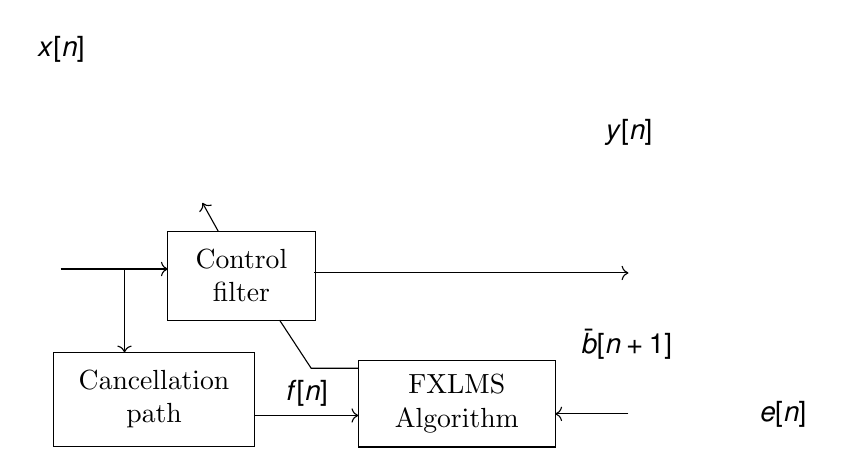
\begin{tikzpicture}
\draw  (-2.9,0.98) rectangle node[text width=2.5cm,align=center] {\textrm{Cancellation \\ path}}(-0.35,-0.21);
\draw  (0.97,0.88) rectangle node[text width=2.5cm,align=center] {\textrm{FXLMS Algorithm}} (3.47,-0.22);
\draw  (-1.45,2.52) rectangle node[text width=1.5cm,align=center,fill=white] {\textrm{Control filter}} (0.42,1.39);
\draw[->] (-0.35,0.18) -- node[above]{$f[n]$} (0.97,0.18);
\draw [->](-2,2.03) -- (-2,0.98);
\draw [->](-2.81,2.04) node[left,above=2.5]{$x[n]$} -- (-1.45,2.04);
\draw[->] (0.41,1.99) -- (1.25,1.99) -- (4.4,1.99) node[left=2.5,above=1.5]{$y[n]$};
\draw (0.97,0.78) -- (0.37,0.78) --node[above=0.55,right=3.5]{$\bar{b}[n+1]$} (-0.03,1.39);
\draw [->](-0.81,2.52) -- (-1.01,2.88);
\draw[->] (4.4,0.2) -- node[above=8,right=2]{$e[n]$} (3.47,0.2);
\end{tikzpicture}
}

%\vspace{-2mm}
%\begin{equation*}
%	b_j[n+1] = b_j[n] - 2\mu e[n]f[n-j]
%\end{equation*}
 
\vspace{3mm}
%\begin{centering}
%	\includegraphics[width=\textwidth]{figures/CombinedSystem2.pdf}
%\end{centering}


It is combined with a linear Wiener filter, allowing prediction of future samples. 
\\ The performance of the predictor is evaluated by calculating Prediction Gain ($PG$), which i the ratio between the signal and the error variance in dB. A larger $PG$ is better. 
\\


%\vspace{-2mm}
%\begin{equation*}
%	PG = 10 log_{10}\bigg(\frac{\sigma^2_x}{\sigma^2_\varepsilon}\bigg)
%%\end{equation*}

\resizebox{1\columnwidth}{!}{
	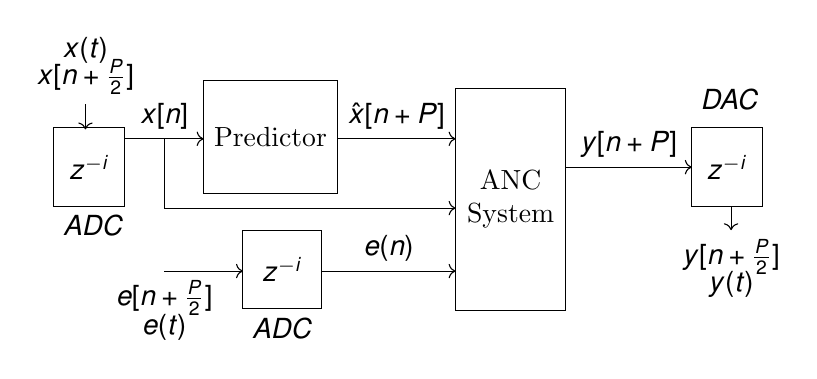
\begin{tikzpicture}
	\draw  (-3.7,1.5) rectangle node {$z^{-i}$} (-4.6,0.5);
	\draw (-4.1,0) node[above]{$ADC$} ;
	\draw (-1.7,-1.3) node[above]{$ADC$} ;
	\draw  (-2.7,2.1) rectangle  node[align=center] {\textrm{Predictor}} (-1,0.66) ;
	
	\draw  (0.5,2) rectangle node[text width=1.5cm,align=center] {\textrm{ANC System}}(1.9,-0.82);
	\draw  (3.5,1.5) rectangle node {$z^{-i}$}(4.4,0.5);
	\draw (3.98,1.6) node[above]{$DAC$} ;
	
	\draw [->](-3.7,1.36)  -- (-2.7,1.36);
	
	
	\draw [->](-1,1.36)  -- node[above]{$\hat{x}[n+P]$}  (0.5,1.36);
	\draw [->](1.9,1) -- node[above]{$y[n+P]$} (3.5,1);
	
	\draw [->](-4.2,1.8) node[above]{$x[n+\frac{P}{2}]$} -- (-4.2,1.48);
	\draw (-4.2,2.2) node[above]{$x(t)$} ;
	\draw [->](4,0.5)-- (4,0.2) node[below]{$y[n+\frac{P}{2}]$} ;
	\draw [->](-3.2,1.36) node[above]{$x[n]$} -- (-3.2,0.48) -- (0.5,0.48);
	\draw (4,-0.78) node[above]{$y(t)$} ;
	\draw  (-1.2,0.2) rectangle node {$z^{-i}$} (-2.2,-0.8);
	
	
	\draw [->](-1.2,-0.32) -- node[above]{$e(n)$} (0.5,-0.32);
	\draw [<-](-2.2,-0.32)-- (-3.2,-0.32) node[below]{$e[n+\frac{P}{2}]$} ;
	\draw (-3.2,-1.32) node[above]{$e(t)$} ;
	\end{tikzpicture}}
\end{posterbox}

\begin{posterbox}[name=Results,column=1,row=0,height=0.88,span=2]{Simulation Results}
\section*{Results}
\subsection{Prediction Gain}
For the purpose of testing LP prediction gain (PG) shown in \autoref{eq:PG} will be used. 
\begin{equation}\label{eq:PG}
PG = 10 log_{10}\bigg(\frac{\sigma^2_x}{\sigma^2_\varepsilon}\bigg) = 10 log_{10}\bigg(\frac{E\{x^2[n]\}}{E\{\varepsilon^2[n]\}}\bigg)
\end{equation}
where PG is the ratio between the variance of the input signal $x[n]$ and the variance of the prediction error $\varepsilon$ in (dB). The higher the PG the better the prediction is.



\subsection{Determining System Parameters}
The parameters which should be detemined are $fs$, $P$, $N$, $O$, and $M$ using \autoref{eq:PG}.         
The PG of variable $fs$ is shown on \autoref{fig:fsPredict}.

\begin{figure}[H]
	\centering
	\textbf{\textit{Here is going to be a graph of PG determined by fs}}
	\caption{PG }
	\label{fig:fsPredict}
\end{figure}


%These are detemined respectively using a Prediction Gain ($PG$) to find the optimum value. 
The PG of variable $N$, $O$ and $M$ is seen on \autoref{fig:PredictParameters}. 
\begin{figure}[H]
	\centering
	\textbf{\textit{Here is going to be a graph of PG determined by N}}
	\textbf{\textit{Here is going to be a graph of PG determined by O}}
	\textbf{\textit{Here is going to be a graph of PG determined by M}}
	\caption{PG }
	\label{fig:PredictParameters}
\end{figure}

\subsection{Simulation of Feedforward LP FXLMS}

\begin{figure}[H]
	\centering
	\tikzsetnextfilename{DelayRatio}
	% This file was created by matlab2tikz.
%
%The latest updates can be retrieved from
%  http://www.mathworks.com/matlabcentral/fileexchange/22022-matlab2tikz-matlab2tikz
%where you can also make suggestions and rate matlab2tikz.
%
\definecolor{mycolor1}{rgb}{0.00000,0.44700,0.74100}%
\definecolor{mycolor2}{rgb}{0.85000,0.32500,0.09800}%
%
\begin{tikzpicture}

\begin{axis}[%
width=3in,
height=1.75in,
scale only axis,
xmin=0,
xmax=50,
xmajorgrids,
xlabel={Delay [100 $\times$ samples]},
ymin=0,
ymax=70,
ylabel style={yshift=0.3em},
xlabel style={yshift=-0.2em},
ytick={0,10,...,70},
ymajorgrids,
ylabel={Attenuation [dB]},
xticklabel shift={.1cm},
yticklabel shift={.1cm},
axis background/.style={fill=white}
]
\addplot [color=mycolor2,solid,line width=1.5pt,forget plot]
  table[row sep=crcr]{%
2	66.5420250310586\\
4	52.9717264302022\\
6	49.4175149424998\\
8	46.8717703569681\\
10	47.5886347675082\\
12	48.5221420089092\\
14	36.1913078215459\\
16	24.6480360536532\\
18	18.5625963047043\\
20	15.9345988709594\\
22	15.2225924490026\\
24	14.4941735350858\\
26	13.5145912190769\\
28	12.5242379572864\\
30	11.8400523957144\\
32	11.4203165228037\\
34	11.2428861871564\\
36	11.1050592495872\\
38	10.862823901561\\
40	10.6158645117455\\
42	10.3154480278615\\
44	9.97867799972119\\
46	9.61958031033587\\
48	9.31052791122033\\
50	9.08997582022533\\
};
\addplot [color=mycolor1,line width=1.5pt,solid,forget plot]
table[row sep=crcr]{%
	2	25.5751628128288\\
	4	20.0199680852144\\
	6	17.0442763613153\\
	8	15.1060127156582\\
	10	13.7310612019933\\
	12	12.6685774343164\\
	14	11.7903474171974\\
	16	11.0441690144364\\
	18	10.3883064900616\\
	20	9.78797702825996\\
	22	9.23075404560805\\
	24	8.7110676592604\\
	26	8.22176906503967\\
	28	7.77006791263877\\
	30	7.35426684398216\\
	32	6.94907270624338\\
	34	6.5323972441528\\
	36	6.08060777493347\\
	38	5.57101511941803\\
	40	4.99733350616245\\
	42	4.35167702165293\\
	44	3.61433096515684\\
	46	2.757705271237\\
	48	1.74470077738877\\
	50	0.5254168140125\\
};
\end{axis}
\end{tikzpicture}%
	\caption{Attenuation achieved by the system for different system delays.}
	\label{Fig:Reference to noise ratio}
\end{figure}








% At this point in time all results are not yet certain, however we will give an idea of how they are going to turn out.
% As presented in the paper thus far, we know what kind of noise we would like to cancel out and how we want to do it. The following list tells which graph will be used to show the results of the acceptance tests.

% \begin{itemize}
% \item Prediction gain - The difference between the input signal and the estimated signal, measured in dB. Used in the LP part.
% \item A plot comparison of frequency response between: A pure signal, a signal with FXLMS noise attenuation and a signal with LP combined with FXLMS attenuation
% \item An expansion of \autoref{Fig:Reference to noise ratio}: As of now only attenuation is showed, but in the future another graph in the figure will show the attenuation of the FXLMS combined with LP - which should yield better attenuation at larger delays.

% \end{itemize}




%\vspace{5in}
\end{posterbox}

\begin{posterbox}[name=discussion,column=3,row=0,height=0.5]{Discussion}
\large
\begin{itemize}
\item Combining LP with FXLMS has proven through simulations to increase the attenuation of a system, where delays are present. \\
\item The predictor is capable of predicting 14 samples at 48 $k$Hz. When predicting 14+ samples the predicted signal distorts. If the distorted signal is then passed through the FXLMS algorithm the distortion is not attenuated.\\
\item In order to make a real time implementation of the algorithm certain practicalities should be considered. Firstly the error microphone(3) can not be placed inside the users ear. Secondly the computational load of the predictor should be decrease. %Possibly by using a multirate system. %working at a lower sampling frequency as in telecommunications. This could be implemented as a multirate system, to also allow playback of signals with higher fs. 
\end{itemize}

\end{posterbox}

\begin{posterbox}[name=conclusion,column=3,below=discussion,above=bottom]{Conclusion}
	  \begin{itemize}
  	\item The AAU poster theme v. 1.1.0 has been tested with baposter v. 2.0, and it can be downloaded from my AAU website \cite{jknaau} or my personal website \cite{jknsqrt-1}.
  	\item If you find a bug in the AAU theme (and not in the baposter template), please do not hesitate to contact me. There is a FAQ at the baposter website \cite{baposter}, if you should have any problems with it.
<<<<<<< HEAD
  \end{itemize}
  
  
%\begin{figure}
%  	\floatbox[{\capbeside\thisfloatsetup{capbesideposition={left,top},capbesidewidth=4cm}}]{HammingNOP10}[\FBwidth]
%  	{\caption{A test figure with its caption side by side}\label{fig:test}}
%  	{\includegraphics[width=5cm]{name}}
%\end{figure}
=======
  \end{itemize}
>>>>>>> 386cdecef39d26e2fa621022e6bf7b02f6531c34

\end{posterbox}

%\begin{posterbox}[name=Acks,column=3,below=conclusion,above=bottom,,height=0.1]{Acknowledgment}
%	The group would like to thank Søren Bech for lending a pair of Beoplay H8 for testing. 
%\end{posterbox}


\begin{posterbox}[name=refs,column=1,span=2,above=bottom]{References}
\bibliographystyle{plain}
\begin{thebibliography}{1}% Simple bibliography with widest label of 1
\itemsep=-0.01em% Save space between the separation
\setlength{\baselineskip}{0.4em}% Save space with longer lines
\bibitem{HansenSnyder} Colin Hansen and Scott Snyder and Xiaojun Qiu and Laura Brooks and Danielle Moreau  : \emph{Active Control of Noise and Vibration}, CRC Press $2^{nd}$ Edition 2012
\bibitem{SpeechCoding} Wai C. Chu: \emph{Speech Coding Algorithms}, Wiley $1^{st}$ Edition 2013
\end{thebibliography}
\end{posterbox}



\end{poster}

\end{document}
